\documentclass{beamer}
\usepackage{amsfonts,amsmath,oldgerm}
\usepackage{ragged2e}

\usetheme{sintef}

\newcommand{\testcolor}[1]{\colorbox{#1}{\textcolor{#1}{test}}~\texttt{#1}}

\usefonttheme[onlymath]{serif}

\titlebackground*{assets/background}

\newcommand{\hrefcol}[2]{\textcolor{cyan}{\href{#1}{#2}}}

\title{Aula Zero - Programa da Disciplina}
\subtitle{2023.1 - SPOPFDS - Prát. e Ferr. de Desenvolvimento de Software}
\course{Tecnologia em Análise e Desenvolvimento de Sistemas}
\author{\href{mailto:luiz.quirino@ifsp.edu.br}{Luiz \textbf{Quirino}}}
\IDnumber{luiz.quirino@ifsp.edu.br}



\begin{document}
\maketitle

%\begin{frame}
%
%      Este material é produzido utilizando \LaTeX\, baseado na SINTEF Presentation, disponibilizado sob licenciamento \hrefcol{https://creativecommons.org/licenses/by-nc/4.0/legalcode}{Creative Commons CC BY 4.0}
%
%\vspace{\baselineskip}

%In the following you find a brief introduction on how to use \LaTeX\ and the beamer package to prepare slides, based on the one written by \hrefcol{mailto:federico.zenith@sintef.no}{Federico Zenith} for \hrefcol{https://www.overleaf.com/latex/templates/sintef-presentation/jhbhdffczpnx}{SINTEF Presentation}

% This template is released under \hrefcol{https://creativecommons.org/licenses/by-nc/4.0/legalcode}{Creative Commons CC BY 4.0} license
%\end{frame}
\footlinecolor{sintefdarkgreen}
\section{Apresentação docente}

\begin{frame}{Sobre o docente:}
Formação:
\begin{itemize}
\item Pós-graduação em Gestão de Riscos e CiberSegurança - Faculdade Focus
\item Sistemas de Informação - UFMS
\item Gestão de Tecnologia da Informação - Unicesumar
\item Técnico em Informática - Centro Paula Souza
\end{itemize}
Áreas de Interesse:
\begin{itemize}
\item Gestão de Tecnologia da Informação
\item Governança de Tecnologia da Informação
\item Gestão de Riscos e CiberSegurança
\item Desenvolvimento de software
\end{itemize}
\end{frame}

\section{Apresentação da disciplina}

\begin{frame}{Ementa}\justifying
      O componente curricular apresenta as práticas e as ferramentas básicas de
desenvolvimento de software como controle de versão, ambientes integrados de
desenvolvimento e guias de estilo de código, de forma a capacitar o aluno no
desenvolvimento de projetos individuais e em equipe.
\end{frame}

\begin{frame}{Objetivo da disciplina}\justifying
      Descrever e utilizar as principais ferramentas empregadas no desenvolvimento de software como controle de versão, ferramentas de comunicação e redes sociais de desenvolvimento. \newline
      \newline
      Configurar e utilizar ambientes integrados de desenvolvimento e suas ferramentas tais como editor e depurador.\newline
      \newline
      Aplicar as boas práticas de desenvolvimento de software, no que se refere à padronização de código, baseada em guias de estilos. 
\end{frame}

\begin{frame}{Objetivo da disciplina}\justifying
      Desenvolver a capacidade de encontrar soluções para problemas, consultando documentações oficiais, redes sociais para desenvolvedores e outras fontes de informações técnicas. \newline
      \newline
      Conhecer e compreender as principais definições, fundamentos e filosofia do movimento de software livre. Conhecer os aspectos jurídicos do software livre e as licenças de software.\newline
      \newline
\end{frame}

\begin{frame}{Conteúdo Programático}\justifying
      \begin{itemize}
            \item Terminal e Linha de Comando
                  \begin{itemize}
                        \item Shell, Comandos e Navegação,
                        \item Manipulação de Arquivos e Diretórios
                        \item Configuração e Ambiente
                  \end{itemize}
            
            
      \end{itemize}
\end{frame}

\begin{frame}{Conteúdo Programático}\justifying
      \begin{itemize}
            \item Controle de Versão
            \begin{itemize}
                  \item Conceitos básicos
                  \item Modelos centralizado e distribuído
                  \item Introdução ao Git
                  \item Repositórios remotos
                  \item Trabalho em equipe
            \end{itemize}
           
      \end{itemize}
\end{frame}
\begin{frame}{Conteúdo Programático}\justifying
      \begin{itemize}
            \item Ambiente de Desenvolvimento
            \begin{itemize}
                  \item Editores de Textos e IDES
                  \item Configuração e Plugins
                  \item Depuração
            \end{itemize}
           
      \end{itemize}
\end{frame}
\begin{frame}{Conteúdo Programático}\justifying
      \begin{itemize}
            \item “Aprender a Pesquisar”
            \begin{itemize}
                  \item Documentações oficiais
                  \item Redes sociais para desenvolvedores
                  \item Fontes de notícias e informações técnicas
                  \item Sites de perguntas e respostas
            \end{itemize}
           
      \end{itemize}
\end{frame}

\begin{frame}{Conteúdo Programático}\justifying
      \begin{itemize}
            \item Software Livre
            \begin{itemize}
                  \item Filosofia, Cultura e História
                  \item Aspectos Jurídicos
                  \item Contribuição em Projetos
            \end{itemize}
           
      \end{itemize}
\end{frame}
\begin{frame}{Conteúdo Programático}\justifying
      \begin{itemize}
            \item Boas Práticas de Desenvolvimento
            \begin{itemize}
                  \item Padronização
                  \item Guias de estilo de código
            \end{itemize}
           
      \end{itemize}
\end{frame}

\begin{frame}{Bibliografia básica}\justifying
      \begin{itemize}
            \item \textbf{CHACON, Scott; STRAUB, Ben.  \textcolor{sintefdarkgreen}{Pro git. 2. ed.}} New York: Apress, 2014. ISBN 9781484200773. Disponível em: https://git-scm.com/book/en/v2. Acesso em: 19 mai. 2019.
            \item \textbf{SHOTTS JR, William E. \textcolor{sintefdarkgreen}{The linux command line: a complete introduction. 5. ed.}} San Francisco: No Starch Press, 2019. Disponível em: http://linuxcommand.org/tlcl.php. Acesso em: 14 jun. 2019.
            \item \textbf{WARD, Brian. \textcolor{sintefdarkgreen}{ Como o linux funciona: o que todo superusuário deveria saber. 1. ed.}} São Paulo: Novatec, 2015. ISBN 9788575225783.         
      \end{itemize}
\end{frame}
      

\begin{frame}{Bibliografia complementar}
      \begin{itemize}
            \item \textbf{BELL, Peter; BEER, Brent. \textcolor{sintefdarkgreen}{Introdução ao GitHub: um guia que não é técnico.}} São Paulo: Novatec, 2014. ISBN 9788575224144.
            \item \textbf{DIAS, José Carlos Vaz. \textcolor{sintefdarkgreen}{Propriedade intelectual e os dez anos da lei de inovação:
            conflitos e perspectivas.}} Rio de Janeiro: Gamma, 2015.
            \item \textbf{EIRAS, Marcelo; MENDONÇA, Nelson. \textcolor{sintefdarkgreen}{Guia de certificação Linux. 2. ed.}} Rio de Janeiro:
            Brasport, 2004. ISBN 9788574521596.
      \end{itemize}
\end{frame}

\begin{frame}{Bibliografia complementar}
      \begin{itemize}
            \item \textbf{SILVEIRA, Newton. \textcolor{sintefdarkgreen}{Propriedade intelectual: propriedade industrial, direito de autor,
            software, cultivares, nome empresarial. 4. ed.}} São Paulo: Manole, 2011. ISBN
            9788520431696. Disponível em:
            https://ifsp.bv3.digitalpages.com.br/users/publications/9788520431696. Acesso em: 14 jun.
            2019.
            \item \textbf{
            SOMMERVILLE, Ian. \textcolor{sintefdarkgreen}{Engenharia de software. 9. ed.}} São Paulo: Pearson Prentice Hall,
            2011. ISBN 9788579361081. Disponível em:
            https://ifsp.bv3.digitalpages.com.br/users/publications/9788579361081.

      \end{itemize}
\end{frame}

\section{Planejamento}


\begin{frame}[fragile]{Planejamento de aulas}
      \begin{columns}
            \begin{column}{0.5\textwidth}
                  \textbf{Definições da disciplina:}
                  \begin{itemize}
                        \item Total de aulas: 38 
                        \item Aulas semanais: 2 (19 semanas)
                        \item Total de horas: 28,50
                        \item Atividades práticas (divididas em entregas mensais, a partir de setembro)
                        \item Atividades teoricas (discussões em sala)
                        \item Desenvolvimento de projeto final
      
                  \end{itemize}


            \end{column}
            \begin{column}{0.5\textwidth}
                 \textbf{Turma: 324043}
                  \begin{itemize}
                        \item Quintas-feiras: 21:20 - 22:50
                        \item Período: 27/07 - 30/11 (07/12 - IFA)
                        \item Feriados: 07/09 - 12/10 - 02/11
                        \item Eventos: 21/09
                  \end{itemize}
                  
            \end{column}
      \end{columns}
\end{frame}



%\section{Moodle}

%\begin{frame}[fragile]{Auto Inscrição Moodle}
%
%      \textbf{Autoinscrição → \textcolor{sintefred}{Chave: IFSP@2023.2}}
%
%      \begin{figure}[H]
%            \centerline{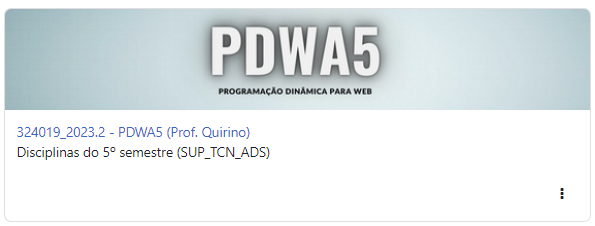
\includegraphics[width=1\textwidth]{assets/aula-tads-pdwa5/moodle_quinta.png}}
%            
%        \end{figure}
%        
%\end{frame}


\section{Avaliações}

\begin{frame}[fragile]\justifying
\frametitle{Sistema de avaliação}
\begin{itemize}
            
            \item Como seremos avaliados:
            \begin{itemize}
                  \item Um trabalho teórico(TT) que atenderá 25\% da nota;
                  \item Um trabalho prático(TP) que atenderá 45\% da nota;
                  \item Atividades avaliativas/participação em aula (AA), contando como 30\% da nota;
            \end{itemize}
            \item Em caso de não obtenção dos critérios mínimos para aprovação, aplicação de IFA por meio de prova teórica, escrita, presencial;
\end{itemize}
\begin{colorblock}[black]{sinteflightgreen}{ATENÇÃO}
      Os trabalhos serão disponibilizados a \textbf{partir da 5ª aula ministrada} na disciplina, contando com documentação disponibilizado pelo docente, ficando aberta para entregas sucessivas no moodle.
      Os trabalhos teórico e prático são interdepentes, sendo a parte teórica / descritiva fudamentada na implementação da atividade prática;
\end{colorblock}

\end{frame}

\begin{frame}[fragile]\justifying
      \frametitle{Sistema de avaliação}
      \begin{itemize}
            \item Média trabalho \[ MT = TP * 0,45 + TT * 0,25\]
            \item Média produtividade \[ MP = \left ( \frac{AA_1 + AA_2 + ... + AA_n}n \right ) * 0,3 \]
            \item Média Final - MF \[MF = MT + MP\]
      \end{itemize}
      
      \end{frame}


\begin{frame}[fragile]\justifying
      \frametitle{Critérios de avaliação}
      Respeitando ao disposto no PPC vigente do curso, no item \textbf{\textit{8. AVALIAÇÃO DA APRENDIZAGEM. }}
      \newline
      \newline
      \textit{Os critérios de aprovação nos componentes curriculares, envolvendo simultaneamente frequência e avaliação, para os cursos da Educação Superior de 
      regime semestral, são a obtenção, no componente curricular, de nota semestral igual ou superior a 6,0 (seis) e frequência mínima de 75\% (setenta e cinco por cento) das
      aulas e demais atividades. }
\end{frame}

\begin{frame}[fragile]\justifying
      \frametitle{Critérios de avaliação}
      \textit{Fica sujeito ao Instrumento Final de Avaliação (IFA), o estudante que obtenha, no componente curricular, nota semestral igual ou superior a
      4,0 (quatro) e inferior a 6,0 (seis) e frequência mínima de 75\% (setenta e cinco por cento) das aulas e demais atividades. O estudante que realizar o Instrumento Final de
      Avaliação, para ser aprovado, deverá obter a nota mínima igual a 6,0 (seis). A nota final considerada, para registros escolares, será a maior entre a nota semestral e a nota do
      Instrumento Final de Avaliação (IFA). 
      \newline
      \newline
      É importante ressaltar que os critérios de avaliação na Educação Superior primam pela autonomia intelectual.}
\end{frame}

\section{Conduta ética}
\begin{frame}
\frametitle{Termos de Conduta}
      \begin{itemize}
            \item Trabalhos e provas devem ser feitas INDIVIDUALMENTE;
            \item Cada estudante tem responsabilidade sobre cópias de suas implementações e provas, mesmo que parciais;
            \item Não faça implementeções em grupo e não compartilhe programas ou trechos de programas;
            \item Você pode consultar seus colegas para esclarecer dúvidas e discutir idéias sobre implementações, mas NÃO copie programas!
            \item Implementações e provas consideradas plagiadas terão nota ZERO;
            \item O estudante que se envolver em DOIS CASOS DE PLÁGIO estará automaticamente REPROVADO na disciplina.
      \end{itemize}
\end{frame}

\section{Informações sobre os slides}

\footlinecolor{sintefyellow}
\begin{frame}
      
      \begin{itemize}
            \item Slides com rodapé em vermelho foram adicionados após a aula dada;
            \item Slides com rodapé em amarelo foram atualizados  após a aula dada.
      \end{itemize}
\end{frame}

\footlinecolor{sintefred}
\begin{frame}[fragile]{Imagem do dia}

        \begin{figure}[H]
            \centerline{
\includegraphics[width=0.5\textwidth]{assets/imagem-do-dia/primeiro-dia-aula.jpg}}
            
        \end{figure}
\end{frame}


\footlinecolor{}

\backmatter
\end{document}
